\mychapter{XBee PRO S3B 900HP}
\label{Cap:Xbee}

O módulo XBee adquirido pelo projeto SpaceVANT para a implementação da rede multi VANTs foi o modelo XBee PRO S3B 900HP fabricado pela Digi Internation\textsuperscript{\texttrademark}. Esse capítulo descreve as especificações técnicas, método de configuração dos módulos e modos de operação como apresentado no guia de usuário do dispositivo. \cite{xbeemanuals3}

\section{Especificações Técnicas}

O guia do usuário do módulo XBee PRO S3B 900HP indica que o mesmo possui um alcance de comunicação de até 610 metros quando em ambiente interno ou urbano e transmitindo a 10 Kb/s. Quando o taxa de transmissão aumenta para 200 Kb/s, o alcance do módulo deve cair pela metade, ou seja, 305 metros. Para ambiente externo e com visada direta, o alcance será de 15.5 quilómetros transmitindo a uma taxa 10 Kb/s e 65 quilómetros quando transmitindo a uma taxa de 200 Kb/s.

O módulo, que ocupa uma volume de aproximadamente 3.66 cm\textsuperscript{3} e pesa entre 5 e 8 gramas, deve ser alimentado com uma fonte de 2.1 até 3.6 volts de corrente contínua, mas para fontes inferiores a 3.0 VDC a performance do módulo pode ser reduzida. A Banda de frequência de operação é selecionável via software e varia entre 902 e 927 MHz. Quanto a \emph{Interface} de dados, UART e SPI estão disponíveis para envio ou requisição de dados do módulo. O XBee PRO S3B 900HP também possui 15 pinos de I/O digital e 4 conversores analógico-digital de 10-bits distribuídos em 20 pinos físicos.

A respeito de rede e segurança, o módulo suporta redes de topologia \emph{mesh}, ponto-a-ponto, estrela ou \emph{peer-to-peer} utilizando Ids de 64 bits para endereçamento. Além disso, estão disponíveis 64 canais de comunicação que podem ser selecionados pelo usuário e opção de criptografia avançada padrão de 128 bits.

\section{Método de Configuração}

A respeito do processo de configuração dos módulos XBee, os parâmetros podem ser consultados e alterados de duas maneiras diferentes: forçando o aparelho a entrar em \emph{AT Command Mode}, solicitando ou enviando os valores do parâmetros do XBee atraves da \emph{interface} de dados, ou fazendo uso de do software XCTU disponibilizado pela Digi International\textsuperscript{\texttrademark}. 

\subsection{AT Command Mode}

A primeira maneira de configurar um módulo XBee seria fazer uso do modo \emph{AT Command Mode} enviando mensagens, de forma serial, requisitando valores de parâmetros ou solicitando alteração de algum parâmetro. É importante alertar que esse modo de configuração só é acessível através do uso da \emph{interface} UART.

Para forçar um modulo XBee a entrar em modo de configuração é necessário enviar um sequência especifica de caracteres, sendo essa sequencia composta por três caracteres de adição (+++). Após receber essa sequência, o módulo retornará `OK' indicando que o mesmo se encontra em \emph{AT Command Mode} aguardando algum comando, caso nenhum comando seja enviado em até um segundo, o modulo sai automaticamente do modo de configuração.

Um vez que o módulo já se encontra em \emph{AT Command Mode}, para solicitar o valor de um determinado parâmetro deve-se enviar a mensagem `AT' acompanhada da sigla do parâmetro que deseja-se obter o valor. Por exemplo, para verificar o valor do parâmetro \emph{Preamble ID} (HP), deve-se enviar o comando `ATHP' e aguardar o retorno do valor atual do parâmetro.

Para alterar o valor de um parâmetro em \emph{AT Command Mode}, deve-se enviar a mensagem `AT' acompanhada da sigla do parâmetro a ser modificado e o novo valor do parâmetro em hexadecimal, o uso de um espaço para separar a sigla do parametro do valor a ser atribuído é opcional. Caso deseja-se modificar o valor do \emph{Preamble ID} para 7FFF, envia-se `ATHP7FFF' ou `ATHP 7FFF'.

\subsection{XCTU Software}

Uma forma mais simples de visualizar e alterar os parâmetros de um módulo XBee é fazer uso do software fornecido pela fabricante do módulo, no caso do XBee PRO S3B 900HP, o XCTU (figura \ref{fig:xctu}) distribuido pela Digi International\textsuperscript{\texttrademark}.

Através do XCTU, pode-se procurar por módulos XBee conectados fisicamente ao computador onde a aplicação está rodando, visualizar e alterar os parâmetros do módulo conectado e até mesmo procurar os outros nós pertencentes a rede a qual o módulo está conectado, bem como visualizar e alterar os parâmetros dos outros nós da rede. 

Além de visualizar e editar paramêtros, o XCTU também possui um modo de console, onde pode-se enviar mensagens ao módulo conectado e visualizar o conteúdo dos mensagens que estão entrando e saindo do módulo, e um modo de visualização de rede, disponível apenas para módulos operando em \emph{API Mode}, onde são mostrados os nós que pertencem a rede do módulo conectado, bem como a topologia da rede.

O XCTU também possui algumas ferramentas para analise da qualidade da rede a qual o módulo XBee está conectada, por exemplo testes de força de sinal e \emph{throughput}, os quais foram utilizados para aferir a qualidade dos \emph{links} formados pelos XBee nesse trabalho.

\section{Modos de Operação}

O módulo XBee PRO S3B 900HP possui três possíveis modos de operação, sendo eles: \emph{Transparent Mode}, \emph{API Mode} e \emph{AT Command Mode}, utilizado exclusivamente para configuração do módulo e previamente explicado.

\subsection{Transparent Mode}

O \emph{Transparent Mode} é o modo de operação padrão do XBee e é obrigatório o uso da \emph{interface} UART ao utilizar desse modo. Quando funcionando em modo transparente, o módulo receberá dados, continuamente, através da porta UART e quando a quantidade de dados atingir o limite de \emph{bytes}, determinado na configuração do parâmetro \emph{Maximum RF Payload Bytes} (NP), os dados serão organizados em um \emph{frame} pelo próprio XBee e esse pacote é então enviado para o destinatário definido pelos parâmetros \emph{Destination Address High} (DH) e \emph{Destination Address Low} (DL). 

Apesar da facilidade de uso, esse modo de operação é indicado apenas para uso em redes com topologia ponto-a-ponto, onde o destinatário dos pacotes não varia com frequência, pois para mudar o destinatário de um pacote nesse modo de operação será necessário entrar em modo de configuração e alterar múltiplos parâmetros para cada envio. Sendo assim, esse modo nao é adequado para a implementação de uma rede multi VANTs onde um mesmo pacote podera ser enviado para múltiplos nós na rede, por exemplo.

\subsection{API Mode}

Diferentemente do \emph{Transparente Mode}, onde o XBee realiza a operação de criação do \emph{frame} que será transmitido, no \emph{API Mode} o módulo já recebe o frame contendo todas informações como destinatário e tipo de dado, por exemplo, e apenas transmite o \emph{frame} recebido de acordo com as informações do mesmo. Esse modo é compatível com ambas as \emph{interfaces} UART e SPI.

A estrutura do \emph{frame} a ser recebido pelo XBee está ilustrada na figura \ref{fig:apiframe} e contem quatro campos principais. O primeiro \emph{byte} do frame indica apenas o início do mesmo, seguido por dois \emph{bytes} que irão indicar o tamanho do frame, sem contar o \emph{byte} que é utilizado para garantir a integridade do \emph{frame} através de um operação \emph{chesksum} e, por fim, a maior porção do \emph{frame} contém o dado que está sendo transmitido e o identificador daquele tipo de dado.

Esse modo de operação é indicado para redes com topologia \emph{mesh}, pois o destinatário no \emph{frame} está indicado dentro do mesmo, sem a necessidade de configurar o módulo a cada novo envio. Sendo assim, o \emph{API Mode} se apresenta como um modo de operação compatível com o contexto de um rede multi VANTs.\\

Apresentadas as especificações técnicas do módulo XBee PRO S3B 900HP, os modos de operação disponíveis e o ambiente de configuração e testes XCTU, o próximo capítulo descreve o procedimento dos testes realizados para avaliar a viabilidade desse módulo na implementação de uma rede multi VANTs, bem como os componentes utilizados nos testes. 

\begin{figure} 
\center
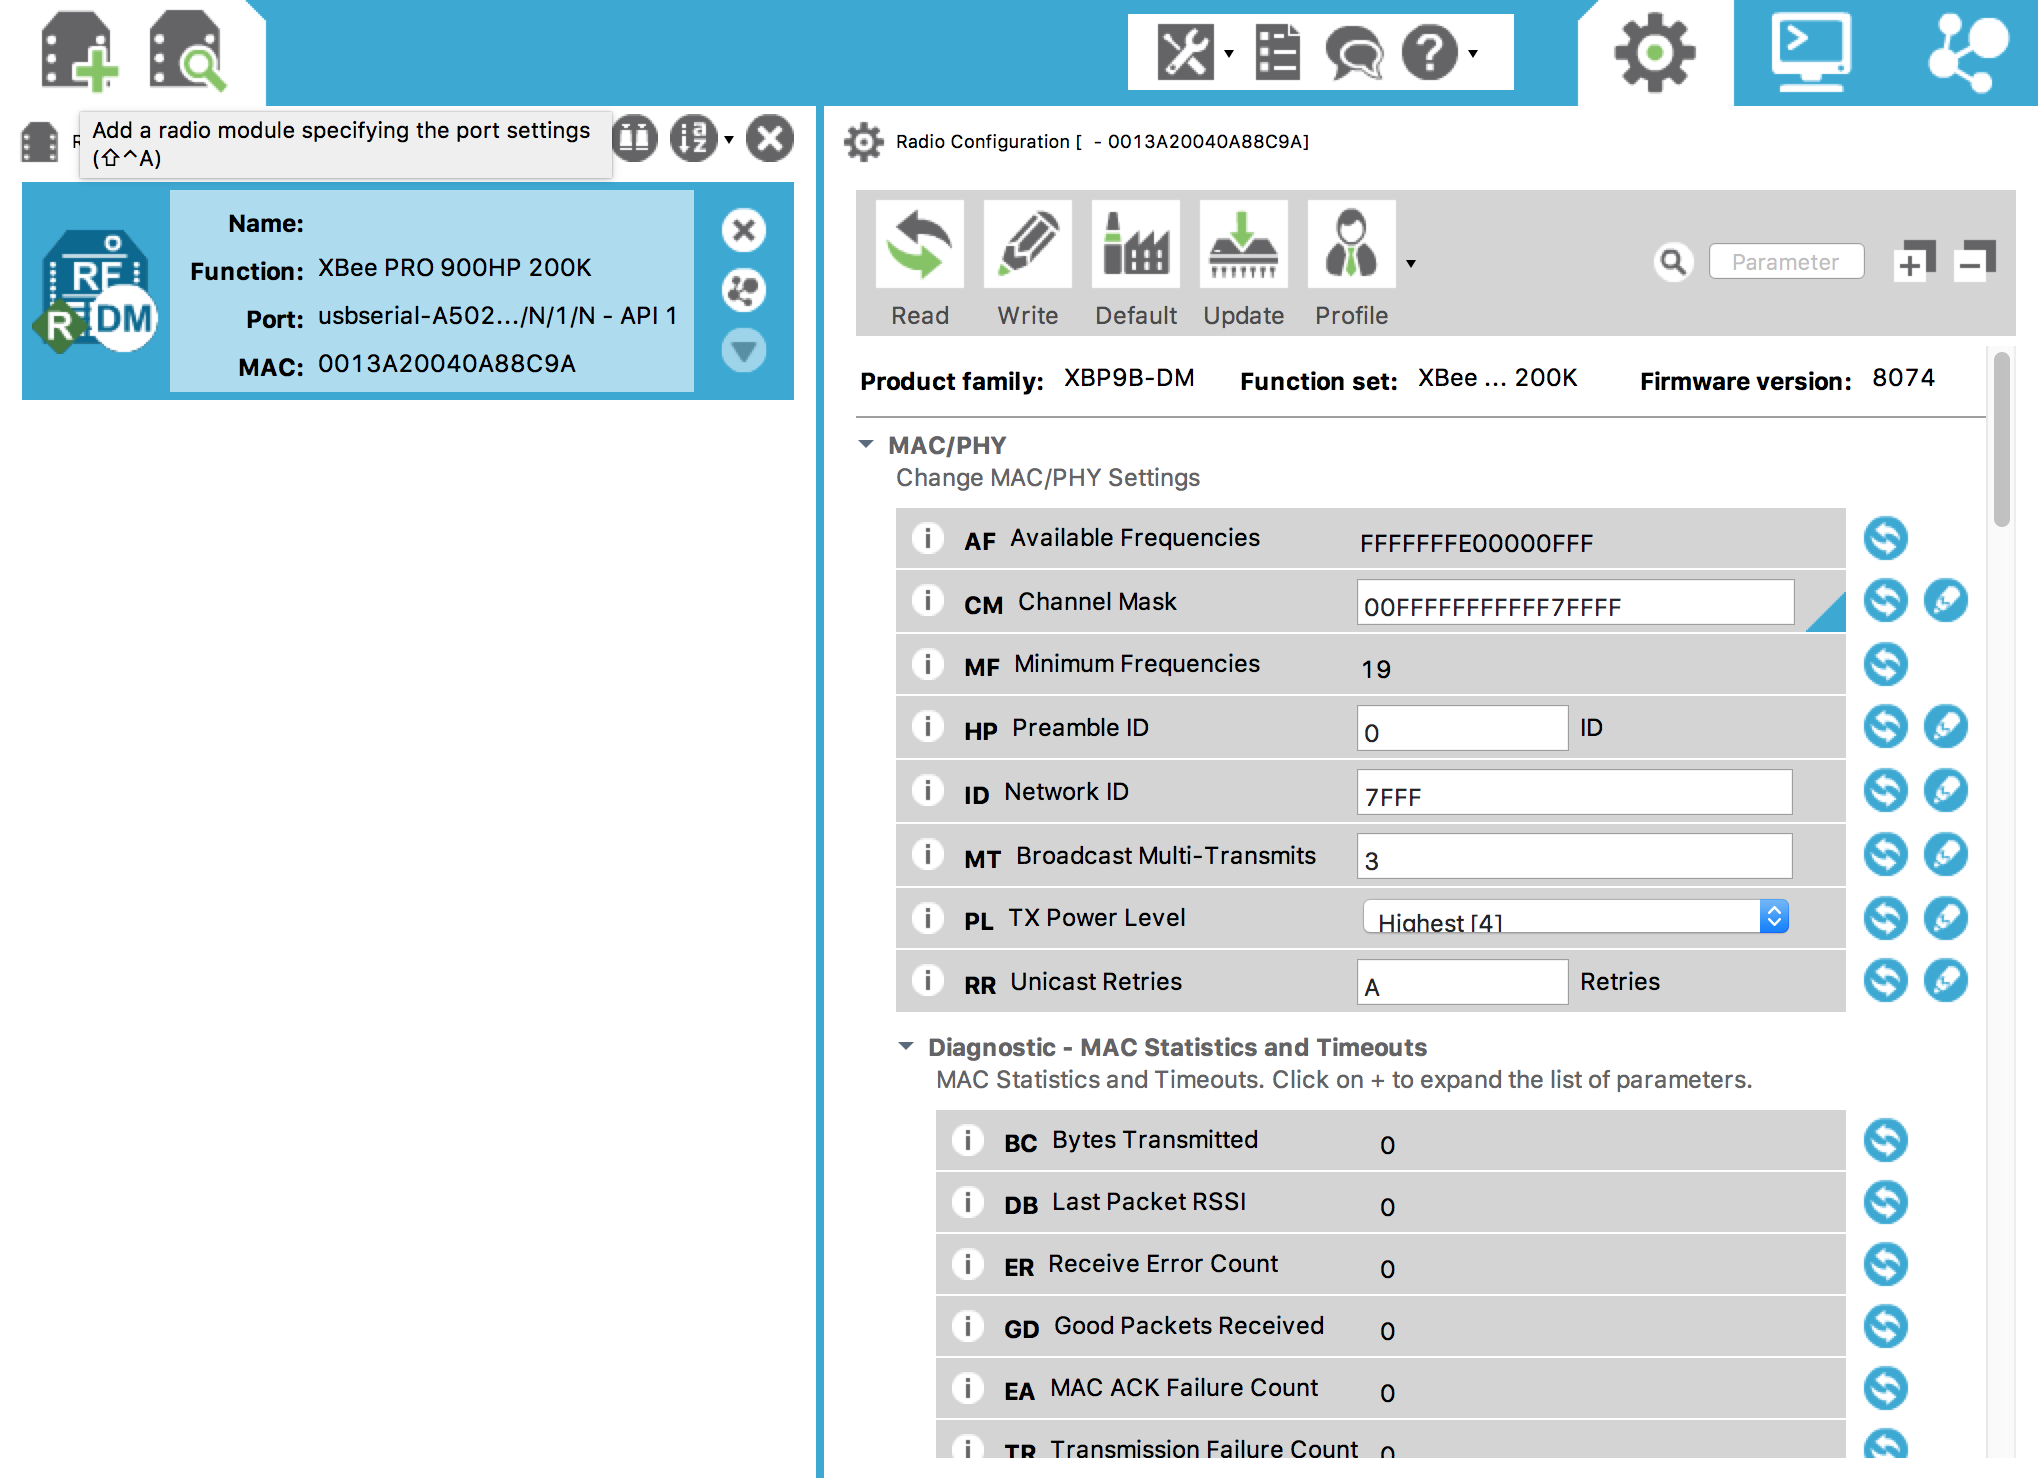
\includegraphics[width=0.7\textwidth]{xctu.png}
\caption{Pagina inicial do software XCTU.} 
\label{fig:xctu}
\end{figure}

\begin{figure} 
\center
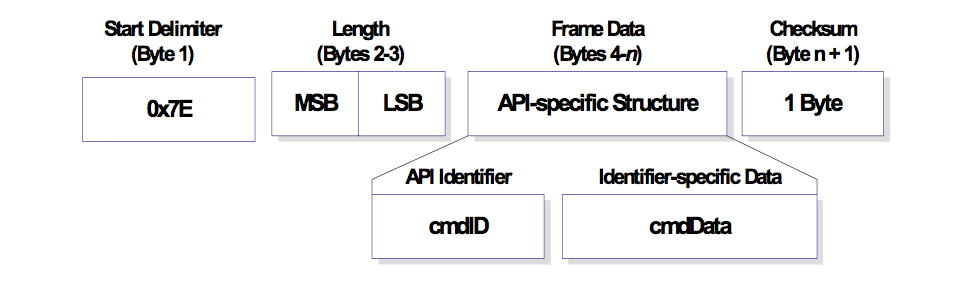
\includegraphics[width=0.7\textwidth]{apiframe.png}
\caption{Estrutura do \emph{frame} no modo API.} 
\label{fig:apiframe}
\end{figure}